%% uctest.tex
%% See accompanying LICENSE file for licensing, history, and copyright
%% information.

% This line is required for LPPL compliance.
\message{You are using a modified uctest.tex}
% Note that if you turn this file into a Derived Work that is not intended as a
% replacement for the original template (i.e. an actual thesis), and you do not
% imply that anyone provides support for your modified version, you may
% distribute it under any license you wish.

\documentclass[11pt]{ucscthesis}
\def\dsp{\def\baselinestretch{2.0}\large\normalsize}
\dsp

% 2010june01 sol katzman:
% package geometry should override the various margin settings from .clo and .cls
% and also eliminates issues where the default papersize is A4
\usepackage[letterpaper, left=1.5in, right=1.25in, top=1.25in, bottom=1.25in, includefoot]{geometry}
% Use PostScript fonts as required by UCSC Dissertation Preparation Guidelines
\usepackage{pslatex}
\usepackage{graphicx}
\usepackage{fullpage} % Package to use full page
\usepackage{parskip} % Package to tweak paragraph skipping
\usepackage{tikz} % Package for drawing
\usepackage{amsmath}
\usepackage{hyperref}
\usepackage{graphicx}
\usepackage{figsize}

\bibliographystyle{unsrt}



\begin{document}

% Declarations for Front Matter

\title{The Elements of Project}
\author{Weiting Zhan}
\degreeyear{2019}
\degreemonth{March}
\degree{Master OF Computer Engineering}
\chair{Professor Roberto Manduchi}
\committeememberone{Professor J. J. Garcia-Luna-Aceves}
\numberofmembers{4} %% (including chair) possible: 3, 4, 5, 6
\deanlineone{Dean John Doe}
\deanlinetwo{Vice Provost and Dean of Graduate Studies}
\deanlinethree{}
\field{Computer Vision}
\campus{Santa Cruz}

\begin{frontmatter}

\maketitle
\copyrightpage

\tableofcontents
\listoffigures
\listoftables

\begin{abstract}
Globally, it is estimated that approximately 1.3 billion people live with some form of vision impairment according to World Health Organization. In this project, the author developed a IOS application and a Android application , both named ISee, for blind user or visually impaired users. Both application takes a picture as input,use Google Firebase MLKit to recognize the character and entities in an image , then read the text or content of the image to user. ISee used the most advanced Optical Character Recognition and Image labeling Application programming interface to help blind or visually impaired user get a some information of the environment. 

\end{abstract}




\end{frontmatter}

\part{First Part}

\chapter{Introduction}
 7,675,600  in the United States reported to have a visual disability in 2016 according to National Federation of the Blind\cite{USBlindStatistics}.Globally, it is estimated that approximately 1.3 billion people live with some form of vision impairment according to World Health Organization.\cite{WHOlindStatistics}

\section{What is Optical Character Recognition?}
Computer store a image as a stream of raw numbers from a camera sensor, typically a array of color intensities of BGR(Blue, green, Red), as show in Fig \ref{Image}. 


\begin{figure}
    \centering
    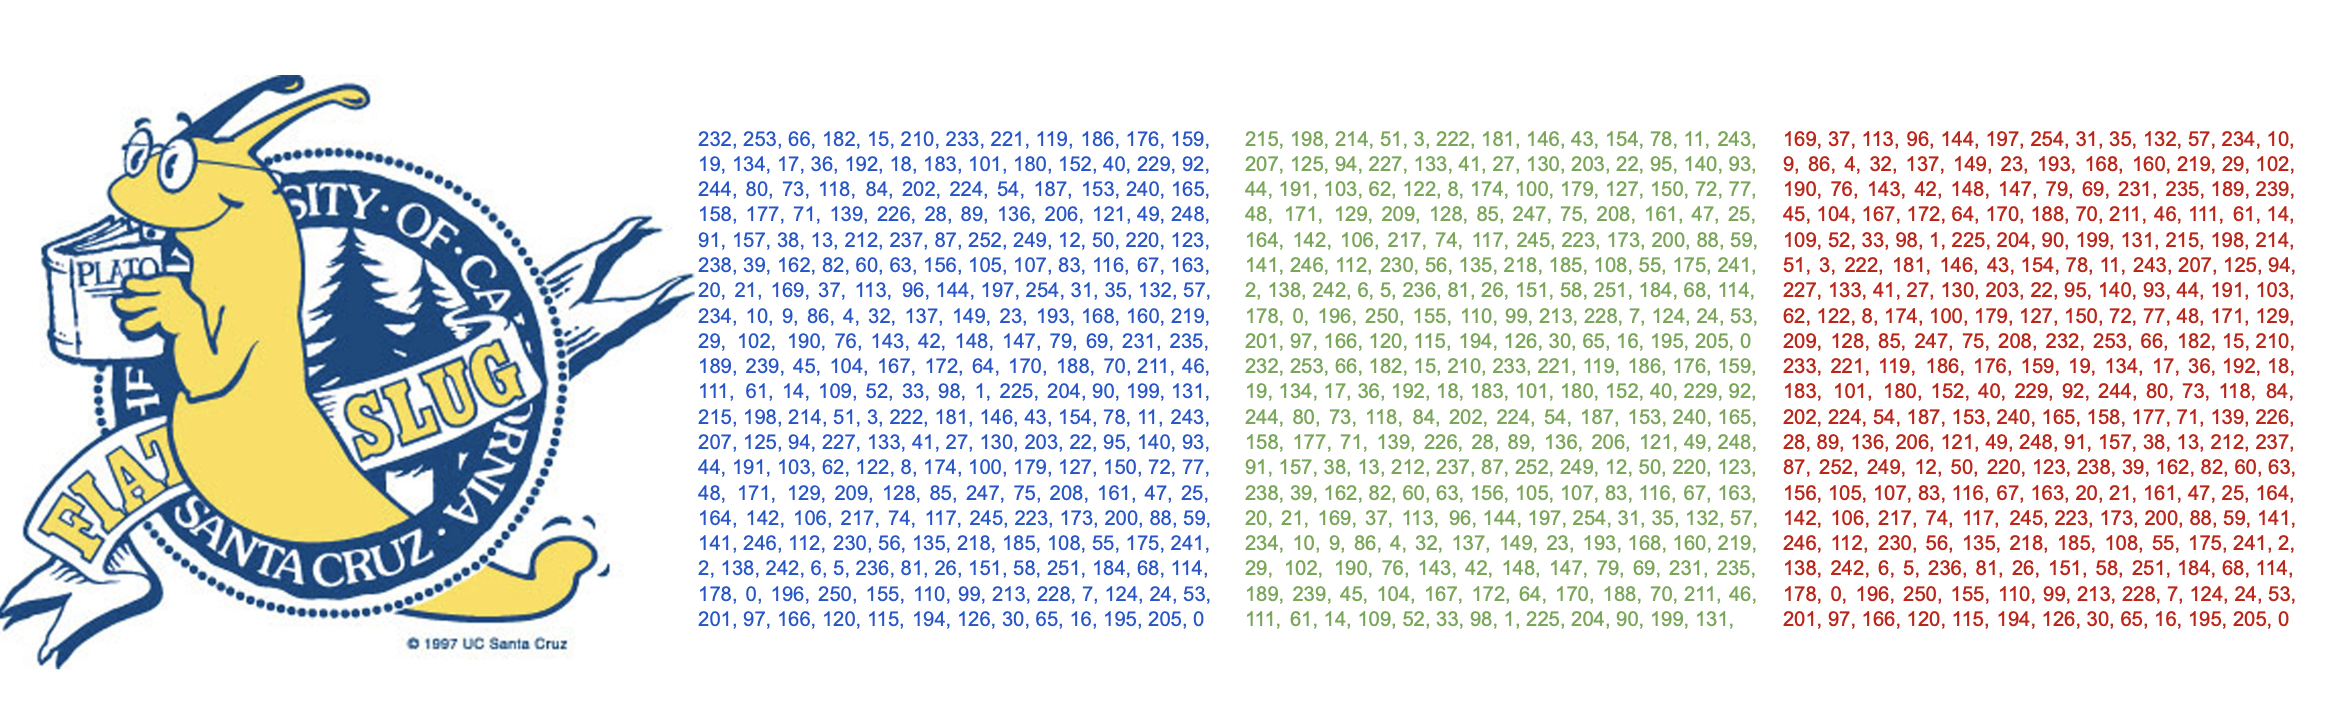
\includegraphics[width =0.8\linewidth]{Fig/image.png}
    \caption{Image stored in computer}
    \label{Image}
\end{figure}


Optical Character Recognition (OCR) transforms images (an array of numbers) into machine-processed text, which is usually encoded using representing scheme. So this become a statistic classification problem\cite{kotsiantis2006machine}\cite{kotsiantis2007supervised}\cite{nickel2015review}, separate one group of numbers (for example, all the images of A in the data set) from another group of numbers (all the images of B in the data set).  
\begin{figure}
    \centering
    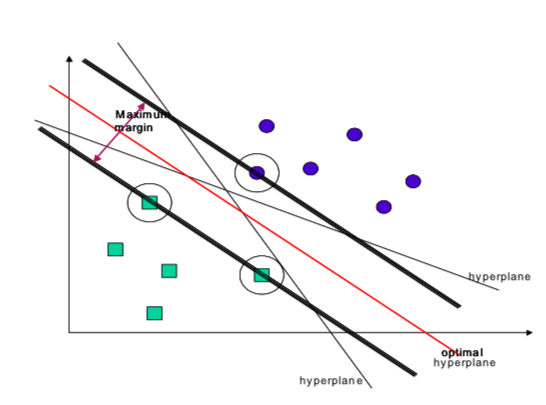
\includegraphics[width =0.5\linewidth]{Fig/SVM.png}
    \caption{Support Vector Machine for Classification\cite{kotsiantis2006machine}}
    \label{SVM}
\end{figure}

Most real-world problems involve non- separable data for which no hyperplane exists that successfully separates the positive from negative instances in the training set. One solution to the inseparability problem is to map the data onto a higher- dimensional space and define a separating hyperplane there. This higher-dimensional space is called the transformed feature space, as opposed to the input space occupied by the training instances. As shown in Fig \ref{SVM}.





Google Cloud Vision \cite{GoogleDocumentTextTutorial} Application Programming Interface(API) , OCR system, is periodically tested on 232 languages in 30 distinct scripts, achieving state of the art accuracy for most of them on image types ranging from scanned documents to casual photos. Currently, a substantial subset of the internally-supported languages are available through the external API.

\begin{figure}
    \centering
    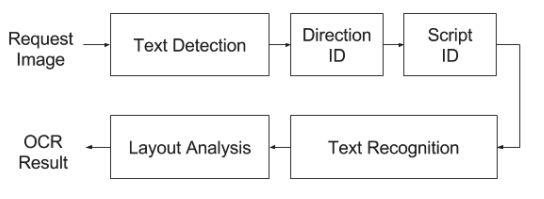
\includegraphics[width =0.8\linewidth]{Fig/googleOCRpipeline.png}
    \caption{Google Cloud Vision API Architecture \cite{GoogleDocumentTextTutorial}}
    \label{Google Document Text Tutorial}
\end{figure}




\section{What is Image labeling?}

Label detection \cite{MLImageLable}is an image annotation feature. This feature predicts the most appropriate labels that describe an image. The feature identifies broad object sets across thousands of different object categories and then returns a label annotation or each detected label in an image. It also returns the following:

Label Identifier: An opaque entity ID for the label, such as "/m/0bt9lr".
Label Description: A textual description of the label, such as "dog."
Confidence Score: A number associated with every returned label annotation, representing the Vision API's assessment of the label's accuracy. Confidence scores range from 0 (no confidence) to 1 (very high confidence).
\begin{figure}
    \centering
    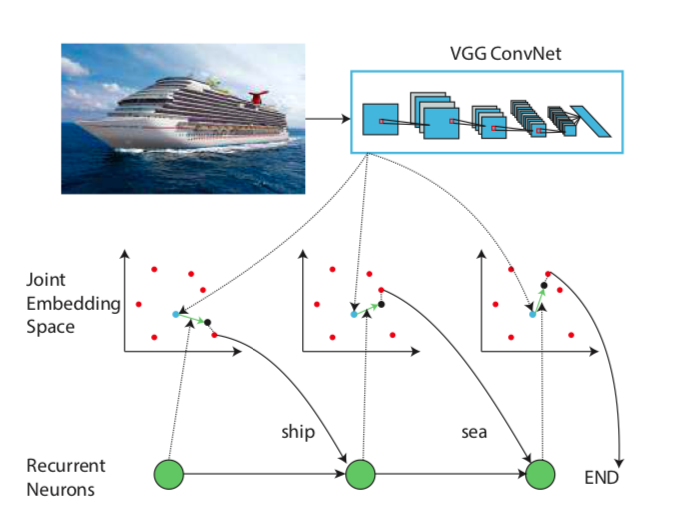
\includegraphics[width =0.8\linewidth]{Fig/RNN- multiclassification.png}
    \caption{ An illustration of the CNN-RNN framework for multi-label image classification.\cite{wang2016cnn}}
    \label{multi-label image classification}
\end{figure}
Multi-label classification can also be achieved by learning a joint image/label embedding.Fig \ref{multi-label image classification} shows that the framework learns a joint embedding space to characterize the image-label relationship as well as label dependency. The red and blue dots are the label and image embeddings, respectively, and the black dots are the sum of the image and recurrent neuron output embeddings. The recurrent neurons model the label co-occurrence dependencies in the joint embedding space by sequentially linking the label embeddings in the joint embedding space. At each time step, the probability of a label is computed based on the image embedding and the output of the recurrent neurons. (best viewed in color)


\section{Optical Character Recognition with Firebase MLkit}
Building a Convolutional Neural Network from scratch and collect enough data \cite{GoogleDatasets} to train the model is a time-consuming and expensive undertaking. It's a huge engineering to get the weight matrix. Good news is that, once the model trained, the weight matrix could be used universally. That said, a number of APIs have recently been developed that aim to allow organizations to glean insights from images without requiring in-house computer vision or machine learning expertise.

Google Firebase ML kit \cite{GoogleMLkit} is Google’s visual recognition API, based on the open-source TensorFlow framework and using a REST API. ML Kit comes with a set of ready-to-use APIs for common mobile use cases: recognizing text, detecting faces, scanning barcodes, labeling images and recognizing landmarks. You simply pass in data to the ML Kit library and it will give you the information you need - all in a few lines of code.

IBM Watson Visual Recognition \cite{IBMclassifier}, part of the Watson Developer Cloud, comes with a large set of built-in classes, but is really built for training custom classes based on images you supply.

Clarif.ai \cite{clarif} is an upstart image recognition service that also uses a REST API. One interesting aspect is that it comes with a number of modules that help tailor its algorithm to particular subjects, like weddings, travel, and food.

With Firebase ML Kit's text recognition\ APIs, you can recognize text in any Latin-based language (and more, with Cloud-based text recognition).

Text recognition can automate tedious data entry for credit cards, receipts, and business cards. With the Cloud-based API, you can also extract text from pictures of documents, which you can use to increase accessibility or translate documents. Apps can even keep track of real-world objects, such as by reading the numbers on trains.

Here, we use Google Firebase MLkit to build application.
\begin{figure}
    \centering
    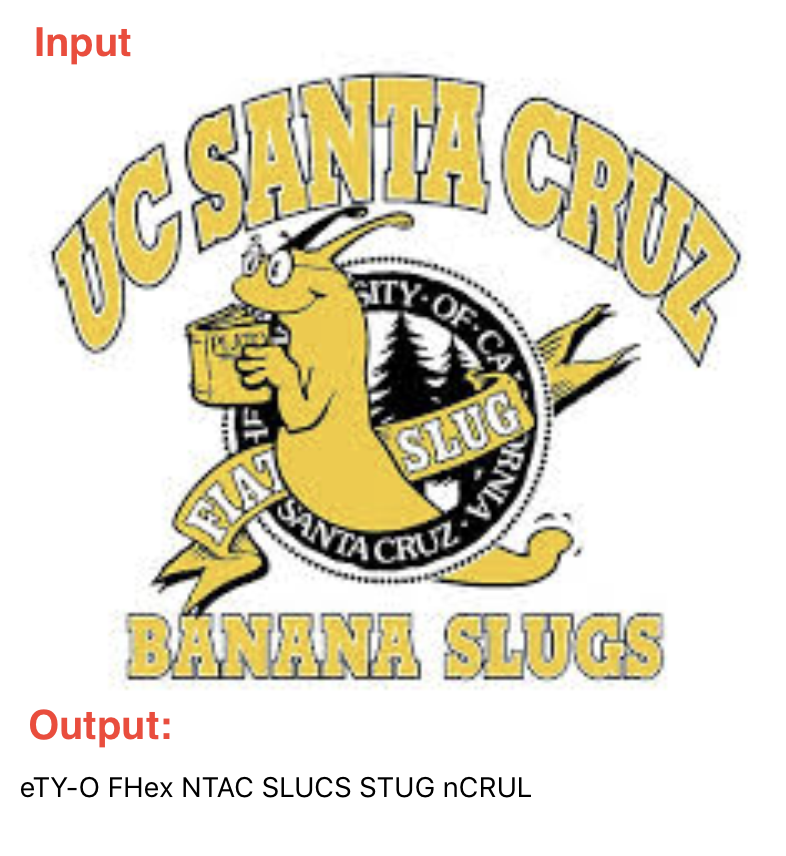
\includegraphics[width =0.4\linewidth]{Fig/OCRdemo.png}
    \caption{Google Firebase MLkit text recognition}
    \label{MLkitOCR}
\end{figure}

\section{Image labeling with Firebase MLkit}
Firebase Image labeling \cite{MLImageLable} gives insight into the content of images. Use the Firebase Image labeling API, you get a list of the entities that were recognized: people, things, places, activities, and so on. Each label found comes with a score that indicates the confidence the ML model has in its relevance. With this information, you can perform tasks such as automatic metadata generation and content moderation.
\begin{figure}
    \centering
    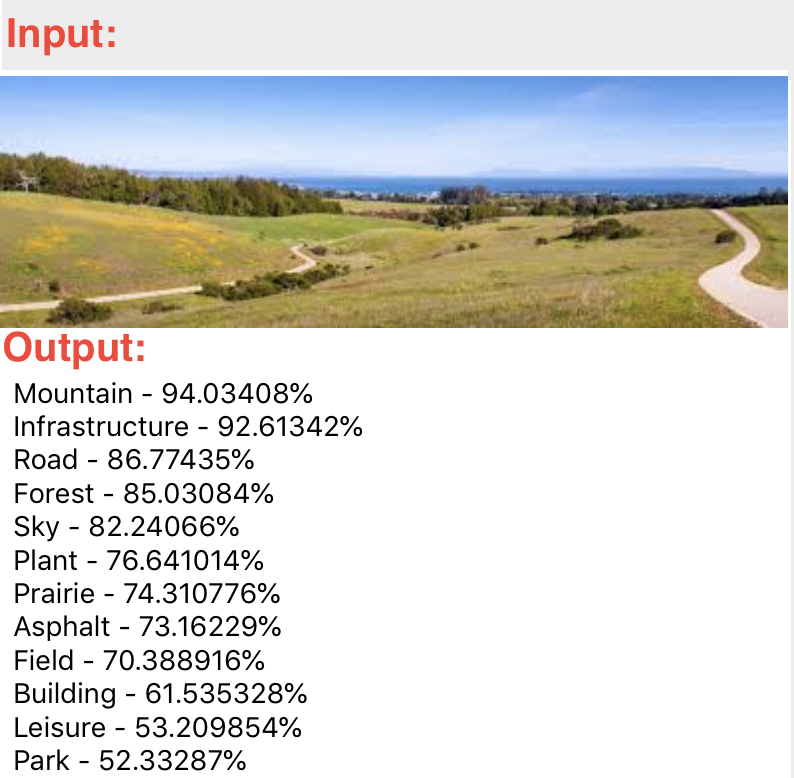
\includegraphics[width =0.5\linewidth]{Fig/Imagelabelingdemo.png}
    \caption{Google Firebase MLkit Image labeling demo}
    \label{MLkitImage labeling}
\end{figure}
The Image labeling on-device offers 400+ labels that cover the most commonly-found concepts in photos, and cloud offers 10,0000+ labels in many categories, as shown in Fig \ref{Firebase MLkitImage labeling}
\begin{figure}
    \centering
    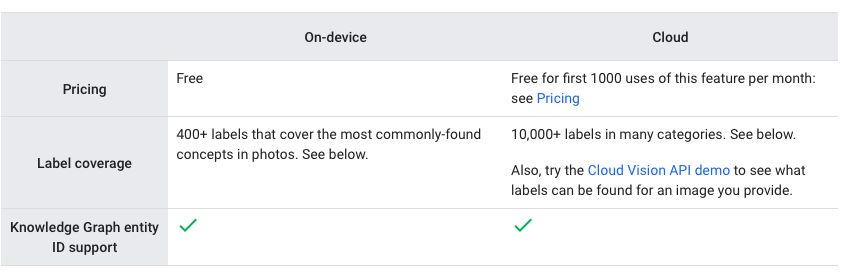
\includegraphics[width =0.5\linewidth]{Fig/FirebaseImageLabeling.png}
    \caption{Google Firebase MLkit Image labeling API\cite{MLImageLable}}
    \label{Firebase MLkitImage labeling}
\end{figure}

\section{Text to Speech API}
With the release of iOS 7, Apple introduced a text to speech API,AVSpeechSynthesizer class\cite{AVSpeechSynthesizer} , that allows developers to add text to speech functionality to an application in a quick and easy way.

Text to speech (TTS)\cite{TTSandroid} makes an android device read the text and convert it to audio out via the speaker. Android TTS supports multiple languages. TTS is a simple but powerful feature. It can also be effectively used in mobile APPs dedicated to visually impaired people or in educational app for kids or can be used in pronunciation learning app, etc. These are some of the ways you can use TTS. Using TextToSpeech enhances interaction between the user and the mobile application. Android TTS was available from version 1.6.





\chapter{Related Work}
\section{Apple Store}
\begin{figure}
    \centering
    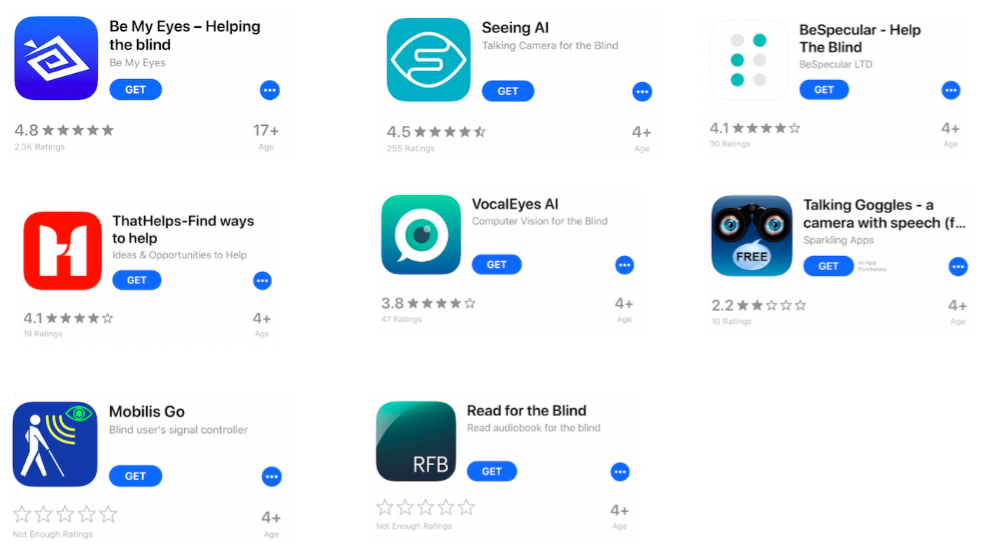
\includegraphics[width =0.8\linewidth]{Fig/AppleBlind.png}
    \caption{Application for blind user in Apple Store}
    \label{Application for blind user in Google Play Store}
\end{figure}

In Apple store,  \textbf{\textit{Talking Googles - a camera with speech}} can recognize images and speaks out what it find. It can recognizes almost any logos, landmarks, books, products, artwork, text. It has video model which continuously check the video stream for identities and speak out.\textbf{\textit{ThatHelps-Find ways to help}}, social network of connecting people who need help and who offer help. It servers as connecting volunteer to blind user.\textbf{\textit{Be My Eyes - Helping the blind}} is also a social network connect volunteer to blind user.\textbf{\textit{Seeing AI}}, developed by Microsoft,use the phone's camera,automatically read what it sees. It can read short text,document,product,person,currency,scene,color,handwriting to user. \textbf{\textit{BlindWays:bus stop navigation}}. help guide blind user to within a cane's distance of an outdoor bus stop sign using permanent landmark clues contributed by volunteers.\textbf{\textit{BeSpecular}}, volunteer help blind by listening to the question sent by blind, or looking at the pictures, and reply with a friendly voice note or text message.\textbf{\textit{Read for the Blind}} create audio books for the blind, by reading books or short articles from magazines, newspapers or any interesting websites.\textbf{\textit{VocalEyes AI, computer vision for the blind}}, created at MIT, identify objects,food,animials,currency and products, as well as read text, detect faces, recognize emotions and describe enviroments using AI. 
 Mobilis Go is designed for blind or visually impaired user. The application uses Bluetooth LE protocol to activate beacons. Activates sound beacons located on objects (like doorways, traffic lights,etc.) Beacons emit sound to help user to navigate.



\section{Google Play Store}
\begin{figure}
    \centering
    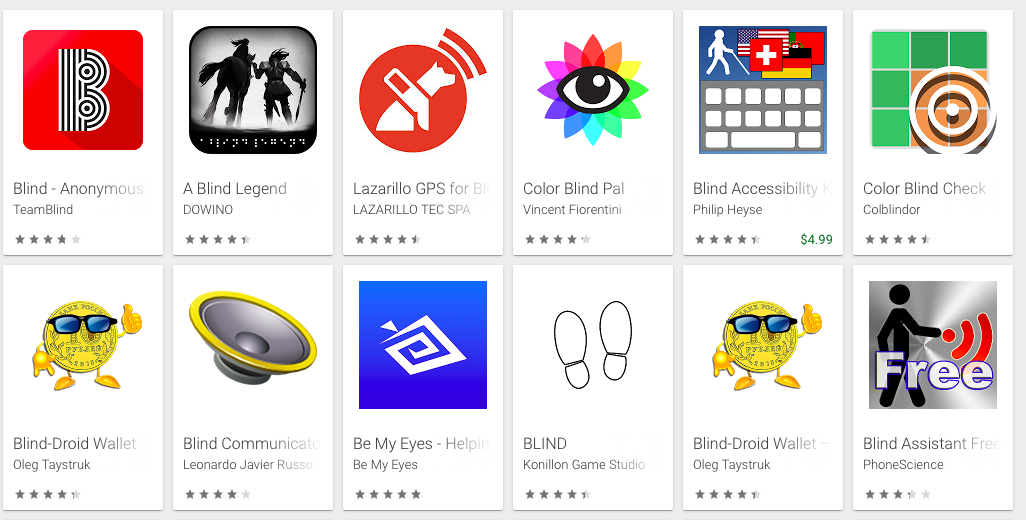
\includegraphics[width =0.8\linewidth]{Fig/GooglePlayStore.png}
    \caption{Application for blind user in Google Play Store}
    \label{Application for blind user in Google Play Store}
\end{figure}
In Google Play store, there are 3 types application for blind user: First,connect blind user with volunteers.\textbf{\textit{Be My Eyes -Helping the blind}} , enables blind to receive live assistance from sighted volunteers. \textbf{\textit{BeSpecular-Help the Blind}}, connect a volunteers to help blind user to identify objects, situations or images. Second, navigation application.\textbf{\textit{Lazarillo GPS}} for Blind use audio messages to tell the visually impaired user about nearby places, the street walking on. \textbf{\textit{Blind Assistant Free}}  turns the phone into a sonar employing a speaker to emit the sound pulses and a microphone to record the return echoes to detect the presence of nearby obstacles and estimate the distance. \textbf{\textit{GetThereGPS nav}} for blind, does not display a map , but tells where is the user and how to get to the destination. \textbf{\textit{Blind Explorer}} is a senatorial guidance system that integrated3D sounds and satellite navigation  technologies to navigate. Third, identify entity for blind user.\textbf{\textit{VIP code Reader}}, is able to detect any QR code or barcode that is present in the camera's field of vision. Blind-Droid Wallet is s an offline paper money recognition.\textbf{\textit{Blind Communicator}} has a voice guide that tells the user everything that it's happening in the device. \textbf{\textit{NowYouSee|A color full world for the color blind}}, created s precisely for the type of color blindness.


In conclusion, there is only 3 applications  \textbf{\textit{Seeing AI}},\textbf{\textit{Talking Googles - a camera with speech}} and \textbf{\textit{VocalEyes AI, computer vision for the blind}},in Apple Store and Google Play Store that designed to describe the environments or surrounding to them just by take a picture of the environments. The API they used is known, so this project offers more options for blind user to choose.



\chapter{Experiment and Result}

Since the application is build on Google Firebase MLkit, the accuracy of the ISee depends on the Google Firebase MLkit, which based on the largest dataset, most advanced algorithm and sufficient computer power.
\section{ISee On IOS device}
\subsection{Optical Character Recognition}

 Use 6 indoor daily images and 6 outdoor daily images to test the Optical Character Recognition on IOS and Android device. As the result shown in Fig.


\begin{figure}
\centering
\SetFigLayout{3}{2}
  \subfigure[Desk]{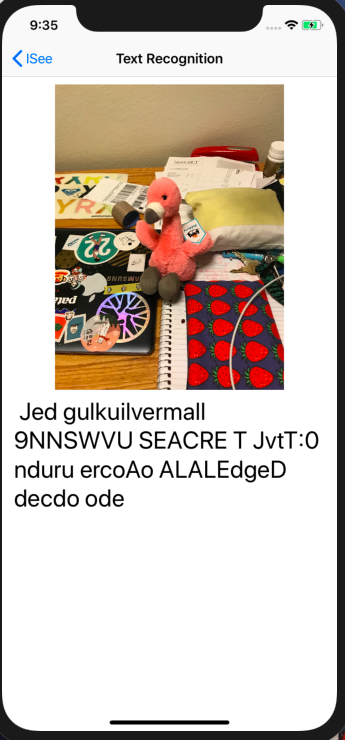
\includegraphics{Fig/FlamingoTextRecognition.png}}
  \hfill
  \subfigure[Presentation]{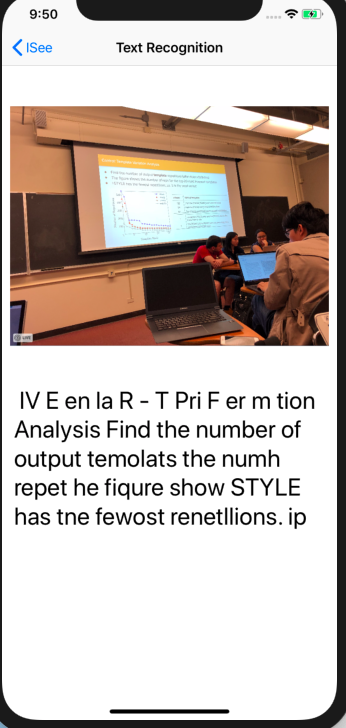
\includegraphics{Fig/ClassTextRecognition.png}}
  \hfill
  \subfigure[Comic]{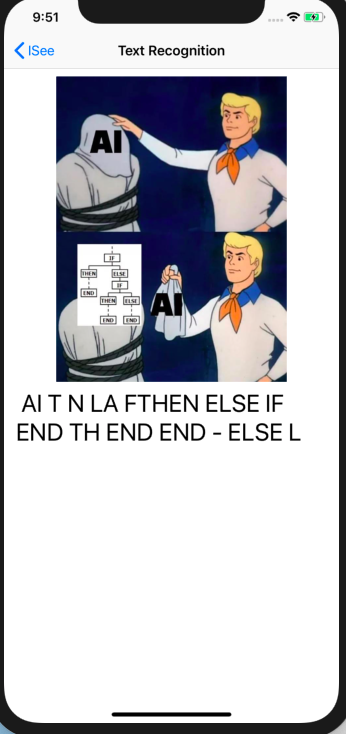
\includegraphics{Fig/AITextRecognition.png}}
  \hfill
  \subfigure[Food]{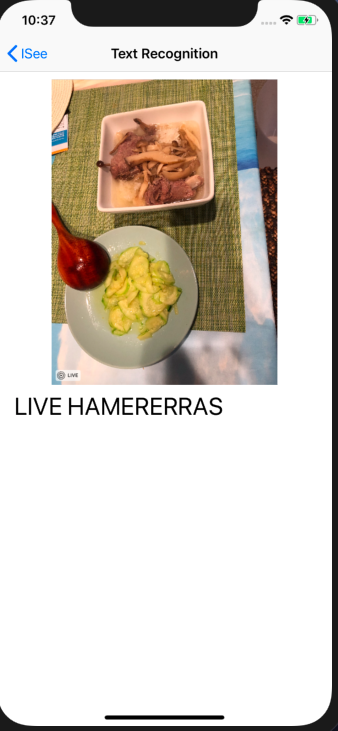
\includegraphics{Fig/foodTextRecognition.png}}
  \hfill
  \subfigure[Dancing Studio]{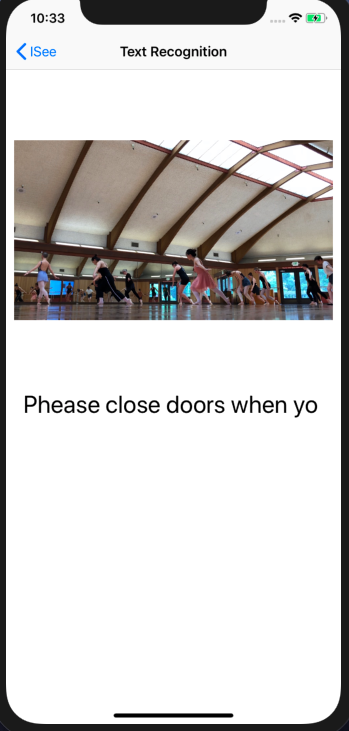
\includegraphics{Fig/BalletTextRecognition.png}}
  \hfill  
  \subfigure[Screen Shot]{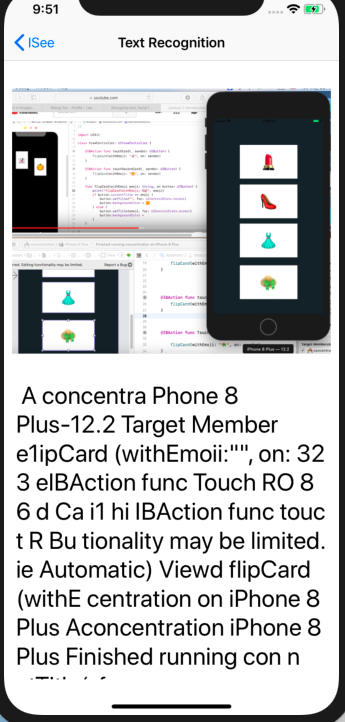
\includegraphics{Fig/ScreenshotTextRecognition.png}}
  \hfill
\caption{Indoor Image Text Recognition on IOS device}
\end{figure}


\begin{figure}
\centering
\SetFigLayout{3}{2}
  \subfigure[Beach]{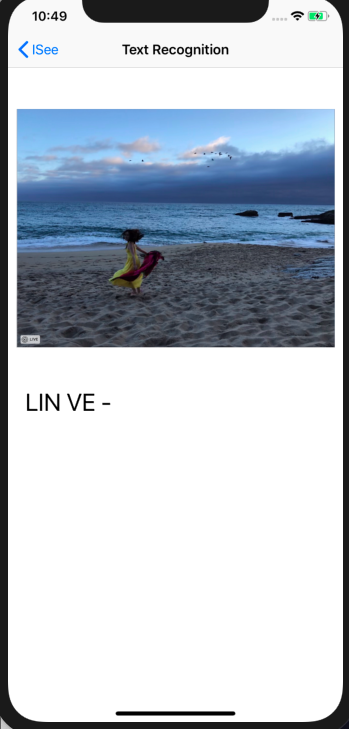
\includegraphics{Fig/BeachTextRecognition.png}}
  \hfill
  \subfigure[Road]{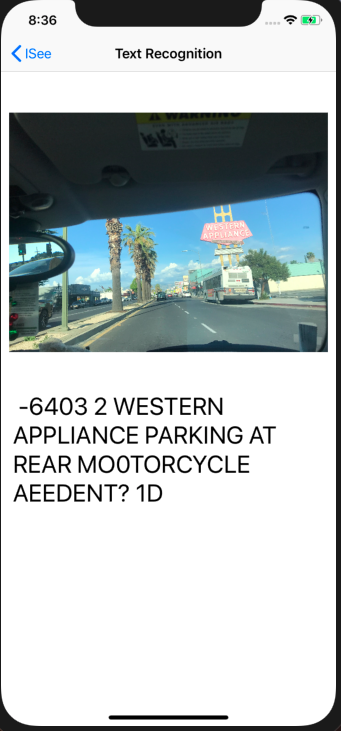
\includegraphics{Fig/carviewTextRecognition.png}}
  \hfill
  \subfigure[
signpost]{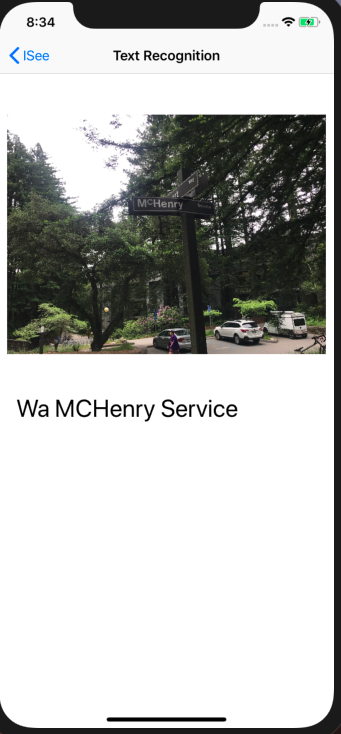
\includegraphics{Fig/signTextRecognition.png}}
  \hfill
  \subfigure[Library Sign]{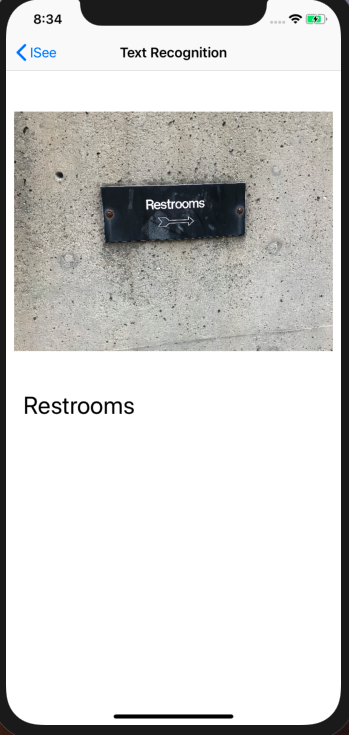
\includegraphics{Fig/RestroomsTextRecognition.png}}
  \hfill
  \subfigure[Parking lot]{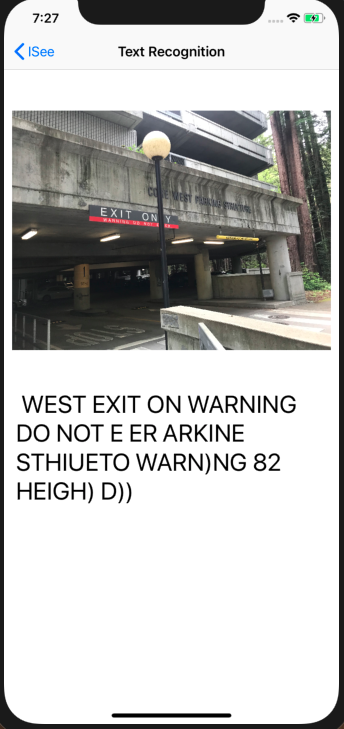
\includegraphics{Fig/parkingTextRecognition.png}}
  \hfill  
  \subfigure[Parking sign]{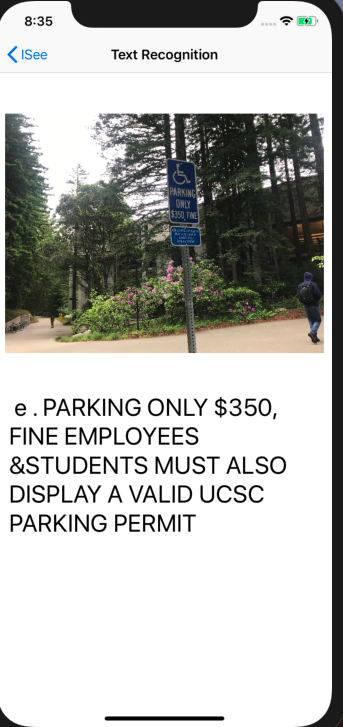
\includegraphics{Fig/parkingsignTextRecognition.png}}
  \hfill
\caption{Outdoor Image Text Recognition on IOS device}
\end{figure}


\subsection{Image labeling}
 Use 10 daily Image to test the Image labeling on IOS and Android device.As the result shown in Fig.

\begin{figure}
\centering
\SetFigLayout{3}{2}
  \subfigure[Desk]{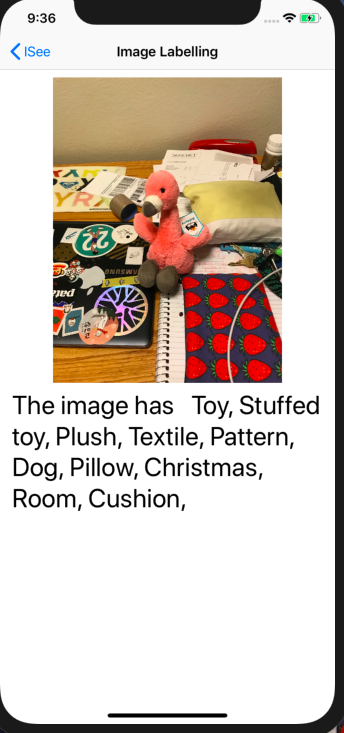
\includegraphics{Fig/FlamingoImageLabelling.png}}
  \hfill
  \subfigure[Presentation]{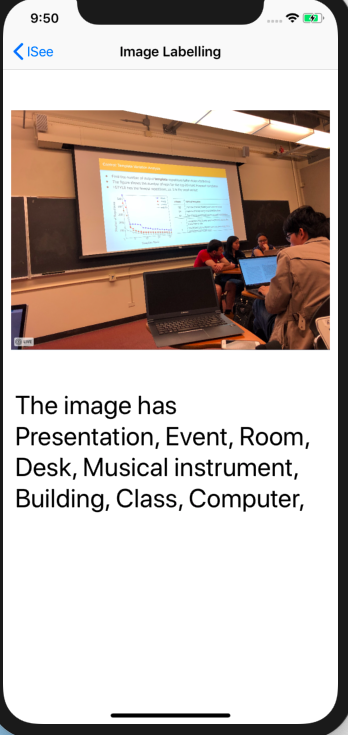
\includegraphics{Fig/ClassImageLabelling.png}}
  \hfill
  \subfigure[Comic]{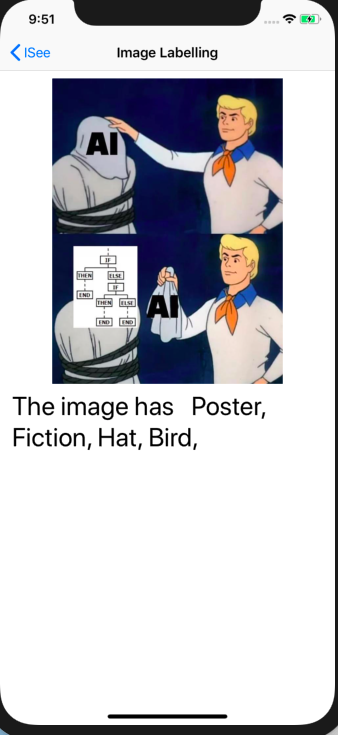
\includegraphics{Fig/AIImageLabelling.png}}
  \hfill
  \subfigure[Food]{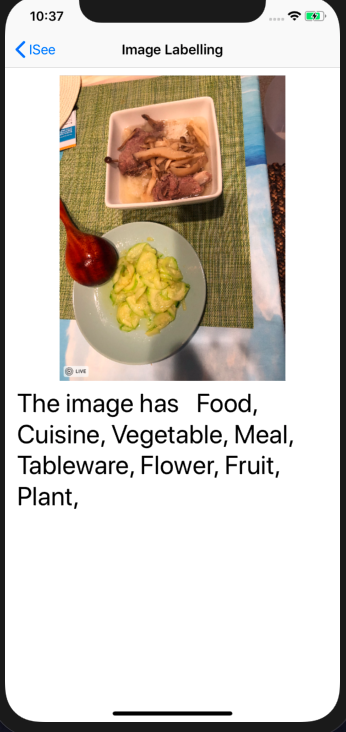
\includegraphics{Fig/foodImageLabelling.png}}
  \hfill
  \subfigure[Dancing Stuidio]{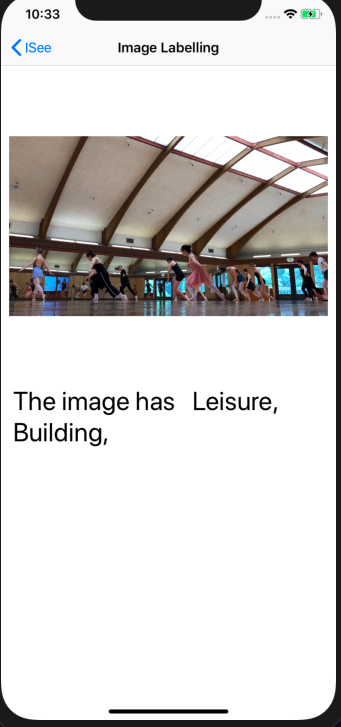
\includegraphics{Fig/BalletImageLabelling.png}}
  \hfill  
  \subfigure[
zebra crossing]{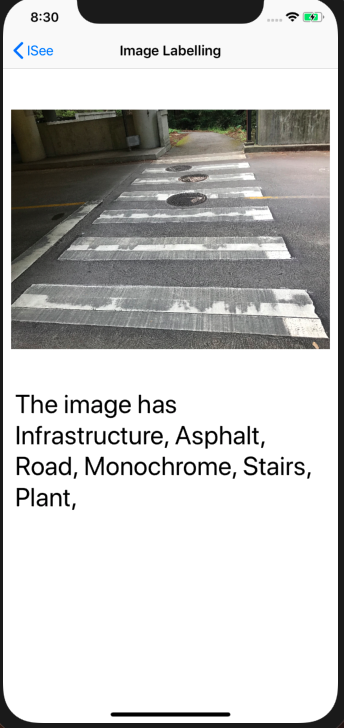
\includegraphics{Fig/RoadImageLabelling.png}}
  \hfill
\caption{Indoor Image Image Labeling on IOS device}
\end{figure}

\begin{figure}
\centering
\SetFigLayout{3}{2}
  \subfigure[Beach]{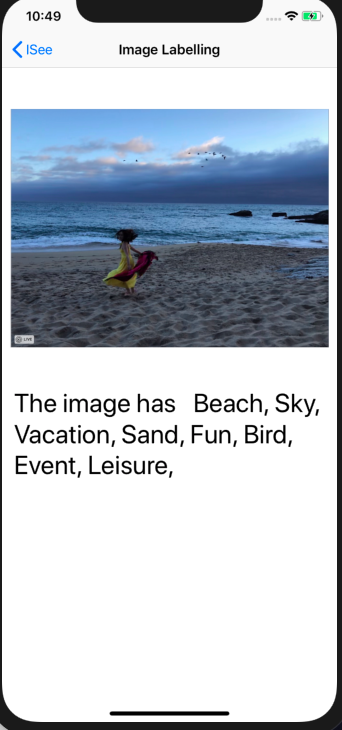
\includegraphics{Fig/BeachImgageLabelling.png}}
  \hfill
  \subfigure[Road]{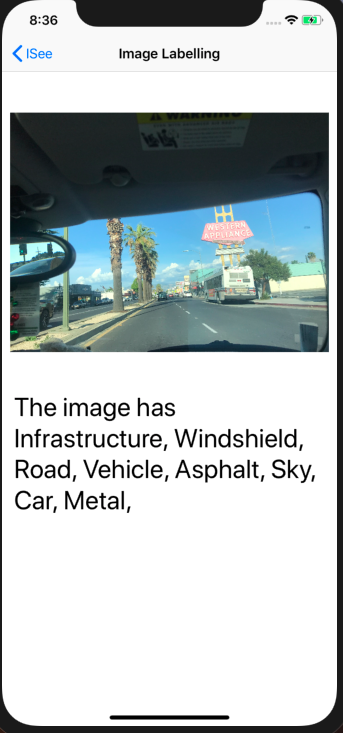
\includegraphics{Fig/carviewImageLabelling.png}}
  \hfill
  \subfigure[signpost]{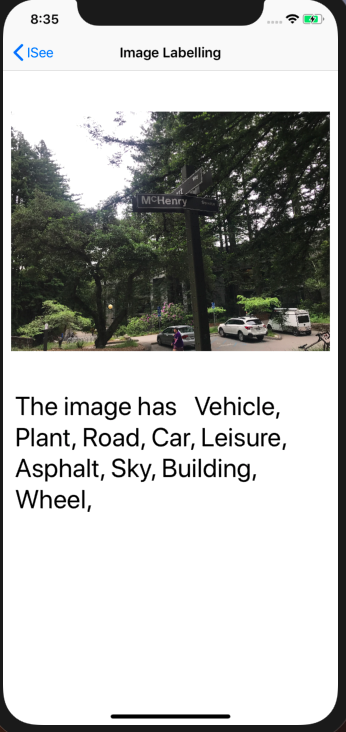
\includegraphics{Fig/signImageLabelling.png}}
  \hfill
  \subfigure[Library sign]{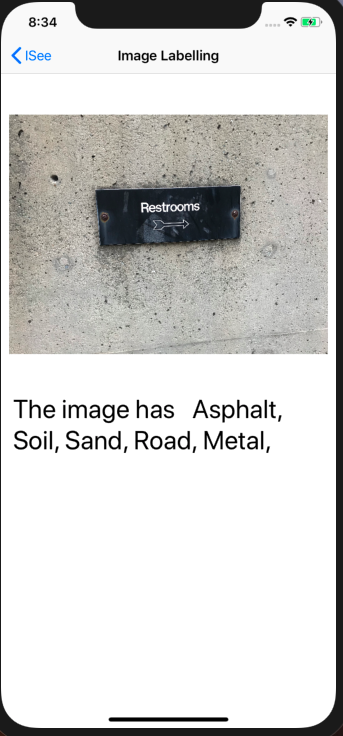
\includegraphics{Fig/RestroomsImageLabelling.png}}
  \hfill
  \subfigure[Parking lot]{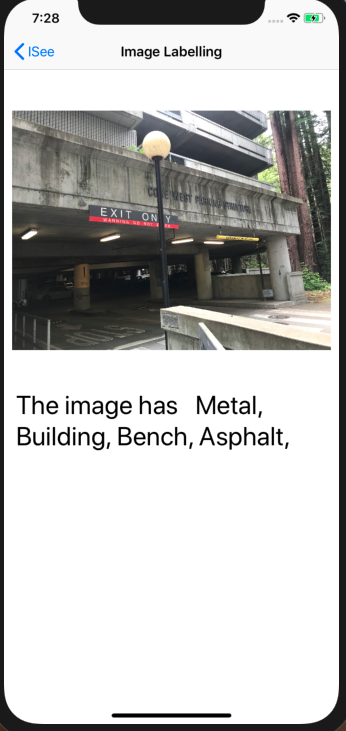
\includegraphics{Fig/parkingImageLabelling.png}}
  \hfill  
  \subfigure[Parking sign]{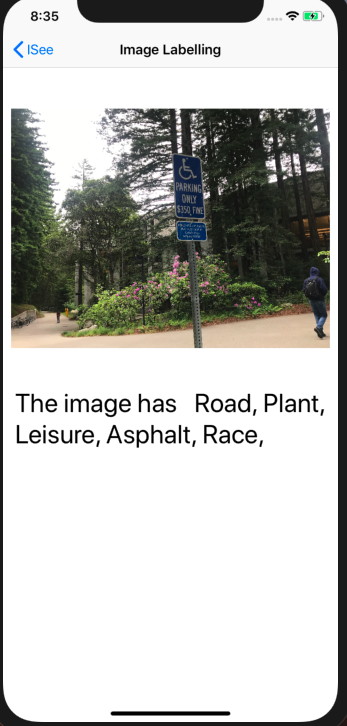
\includegraphics{Fig/parkingsignImageLabelling.png}}
  \hfill
\caption{Outdoor Image Image Labelling on IOS device}
\end{figure}


\subsection{Text to Speech}
For the Text to speech, use the result from Optical character recognition, add a template to the result.

For optical character recognition, if the text are detected, the template will be "the text in the image are + resultOfOCR". otherwise, the template will be "I am unable to detect any text in the image".

For image labeling, the template will be "The image has" + result from Image labeling +" in the image.

Test 10 images from Optical Character Recognition and 10 images from Image labeling. The template works fine and the text to speech works fine.


\section{ISee on Android device}
The application is based on Firebase MLkit \cite{Android}. Use 6 indoor daily images and 6 outdoor daily images to test the Optical Character Recognition on Android device. As the result shown in Fig.

\subsection{Optical Character Recognition}
\begin{figure}
\centering
\SetFigLayout{3}{2}
  \subfigure[Candy letters]{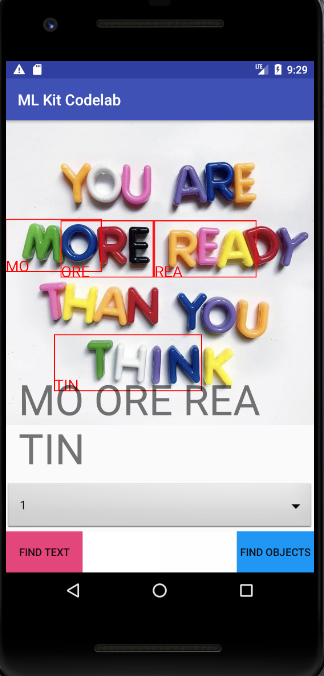
\includegraphics{Fig/androidyouareText.png}}
  \hfill
  \subfigure[SEM image]{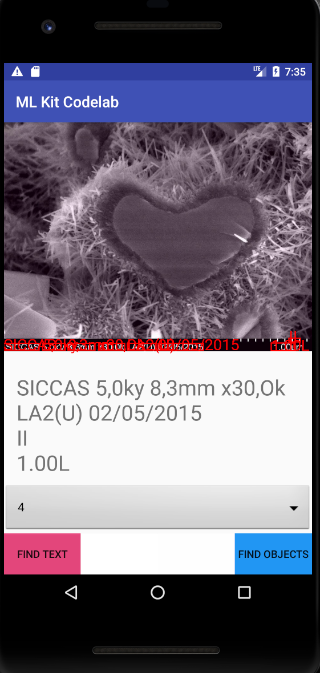
\includegraphics{Fig/andtext2.png}}
  \hfill
  \subfigure[NBA Oracle Arena]{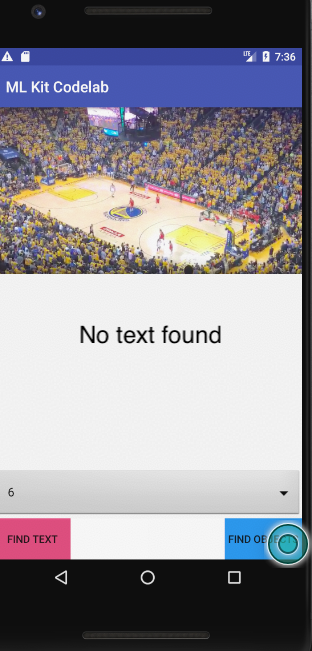
\includegraphics{Fig/androidplaytext1.png}}
  \hfill
  \subfigure[Handwriting]{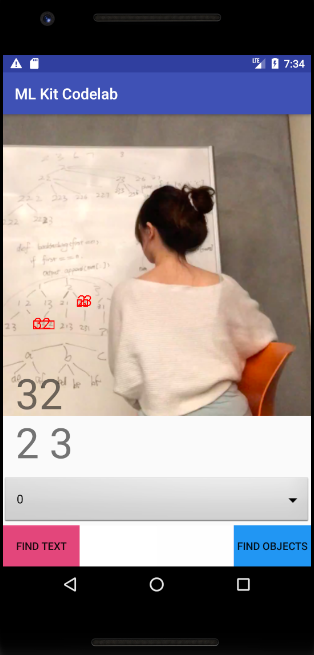
\includegraphics{Fig/andindoortext1.png}}
  \hfill
  \subfigure[slides]{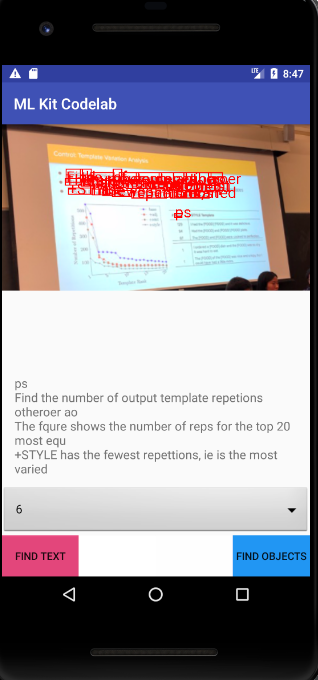
\includegraphics{Fig/andslidestext.png}}
  \hfill  
  \subfigure[Super market]{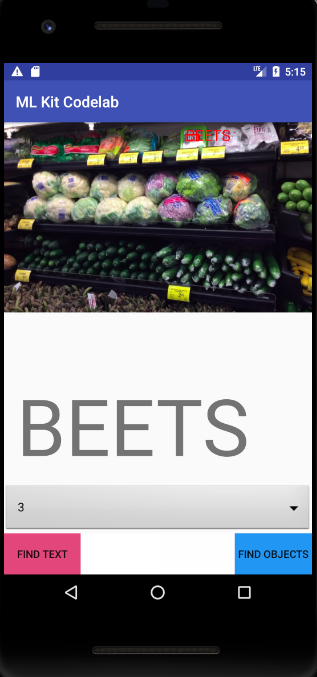
\includegraphics{Fig/andvegT.png}}
  \hfill
\caption{Indoor Image Text Recognition on Android device}
\end{figure}

\begin{figure}
\centering
\SetFigLayout{3}{2}
  \subfigure[Reno sign]{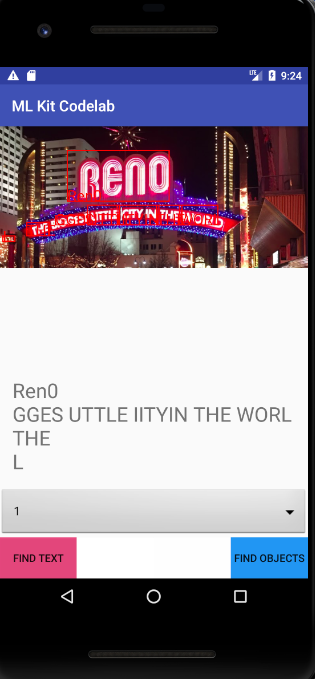
\includegraphics{Fig/androidrenotext.png}}
  \hfill
  \subfigure[Carpools sign]{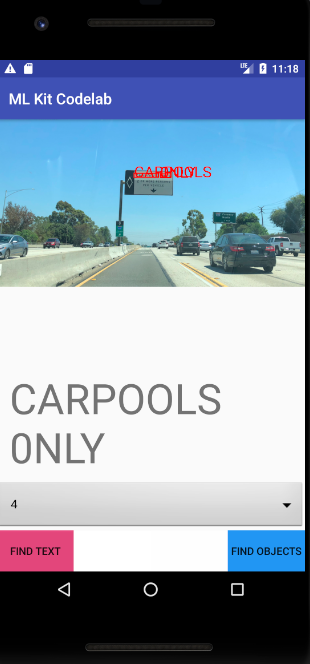
\includegraphics{Fig/an2.png}}
  \hfill
  \subfigure[Farm]{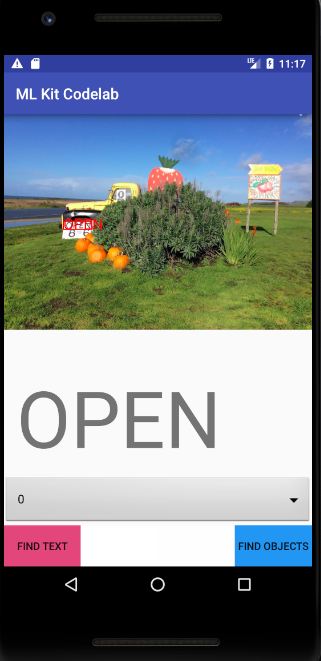
\includegraphics{Fig/an3.png}}
  \hfill
  \subfigure[UCSC sign]{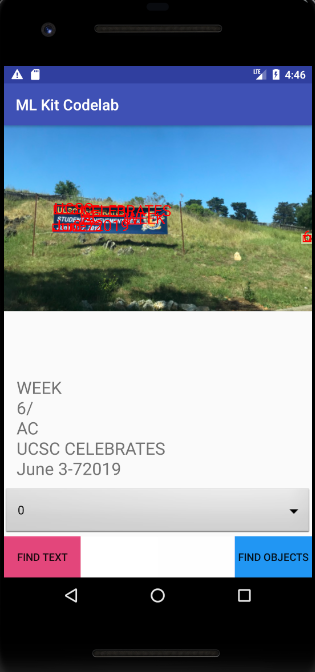
\includegraphics{Fig/anducsct.png}}
  \hfill
  \subfigure[License plate]{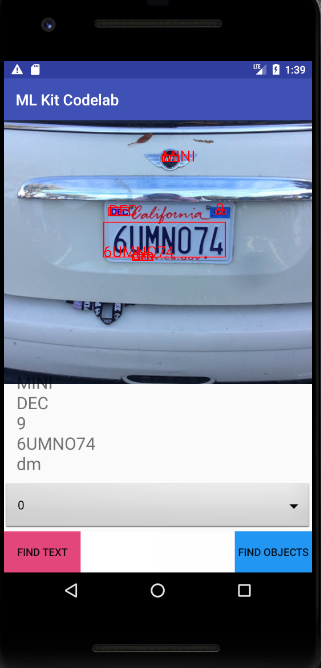
\includegraphics{Fig/an5.png}}
  \hfill  
  \subfigure[Building]{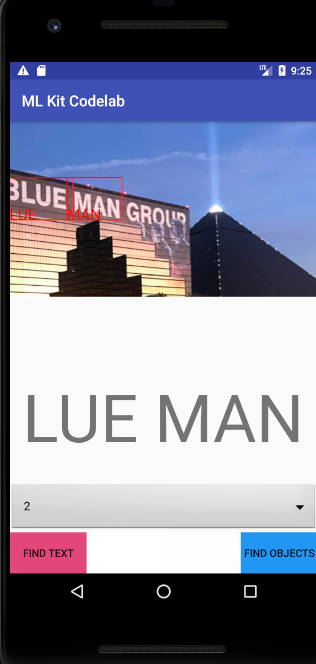
\includegraphics{Fig/androidBluetext.png}}
  \hfill
\caption{Outdoor Image Text Recognition on Android device}
\end{figure}


\begin{figure}
\centering
\SetFigLayout{3}{2}
  \subfigure[candy letters]{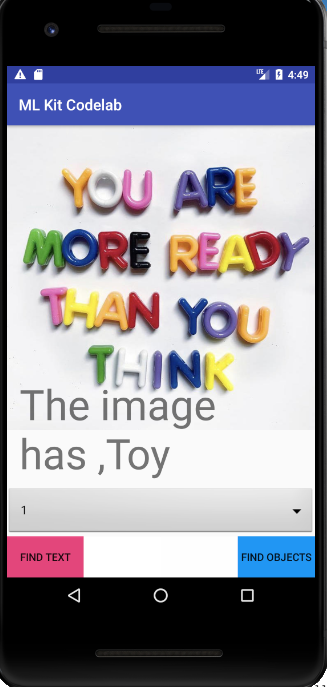
\includegraphics{Fig/andletteri.png}}
  \hfill
  \subfigure[SEM image]{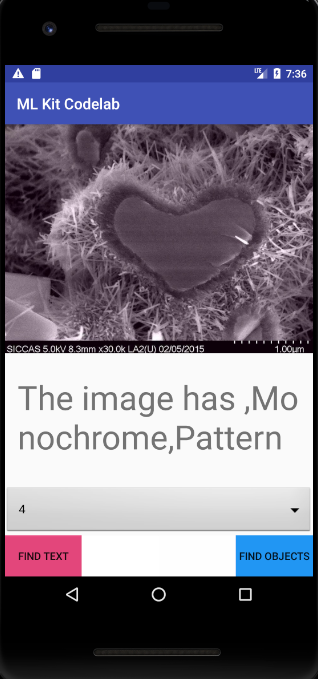
\includegraphics{Fig/andimage2.png}}
  \hfill
  \subfigure[NBA Oracle Arena]{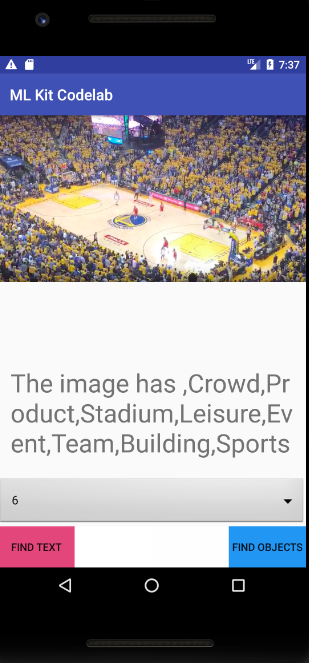
\includegraphics{Fig/androidplayimage.png}}
  \hfill
  \subfigure[Handwriting]{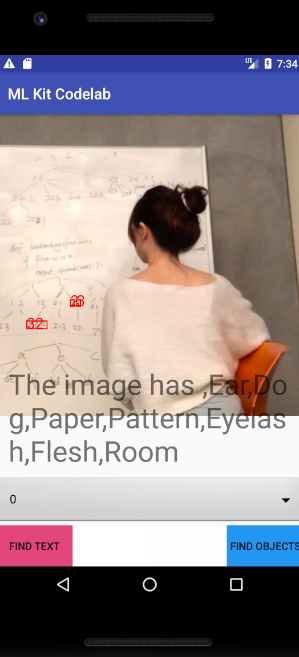
\includegraphics{Fig/andmeimagelable.png}}
  \hfill
  \subfigure[Slides]{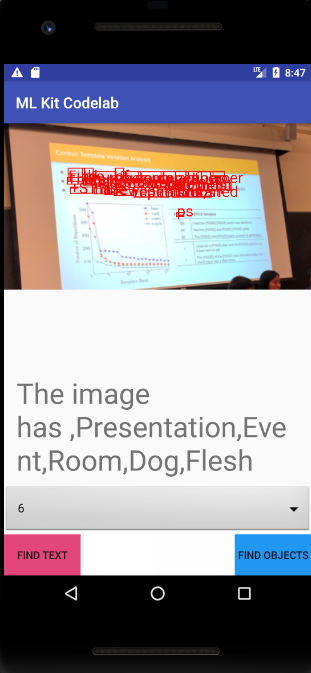
\includegraphics{Fig/andslidesimage.png}}
  \hfill  
  \subfigure[Super market]{\includegraphics{Fig/andvegI.png}}
  \hfill
\caption{Indoor Image Image Labelling on Android device}
\end{figure}
\subsection{Image labeling}


\begin{figure}
\centering
\SetFigLayout{3}{2}
  \subfigure[Beach]{\includegraphics{Fig/androidseaImage.png}}
  \hfill
  \subfigure[Farm]{\includegraphics{Fig/andopeni.png}}
  \hfill
  \subfigure[Sunset]{\includegraphics{Fig/androidsunset.png}}
  \hfill
  \subfigure[UCSC sign]{\includegraphics{Fig/anducsci.png}}
  \hfill
  \subfigure[Licensee plate]{\includegraphics{Fig/andcari.png}}
  \hfill  
  \subfigure[Beach]{\includegraphics{Fig/andSealI.png}}
  \hfill
\caption{Outdoor Image Image Labelling on Android device}
\end{figure}
\subsection{Image labeling}



\subsection{Text to Speech}



\chapter{Conclusion}
The project made an ISee application for blinder user or visually impaired user on IOS device and Android device. ISee can read text and the entity in the image for blind user. The accuracy of the ISee depends on Google Firebase Text recognition API and Image Labeling. The performance of ISee is not enough for navigation, just offer a glimpse of the real world to blind user.


 

\part{Documentation}
The code for the project can be found:
Prerequisites for firebase:
\appendix
\chapter{Compiling}
\section{System Prerequisite for IOS}
\item[iOS 11.4]
\item[Xcode 10.1]
\item[Swift 4.2]
\item[Firebase]

\section{System Prerequistie for Android}
\item[iOS 11.4]
\item[Xcode 10.1]
\item[Java]
\item[Firebase Targets API level 16 (Jelly Bean) or later
Uses Gradle 4.1 or later]

\chapter{Functions}



% %%%%%%%%%%%%%%%%%%%%%%%%%%%%%%%%%%%%%%%%%%%%%%%%%%%%%%%%%
% bibliography

% 2010june01 sol katzman:
% if \nocite is specified, all entries in the bib file are included,
% probably not what you want, so comment out the \nocite and only get the cited references.
%\nocite{*}

% 2010june01 sol katzman:
% this makes the bibliography single spaced, with double spacing between entries
\def\baselinestretch{1.0}\large\normalsize

\bibliographystyle{plain}
\bibliography{uctest}
\begin{acknowledgements}
The author thank Professor Roberto Manduchi and for their feedback and helpful suggestions.

\\
The author thank Hyein Jeong for the data collection in the project.
\end{acknowledgements}

\end{document}